\chapter{Evaluation}

(Joshua)

Die in dieser Arbeit vorgestellte \textit{Travlyn} Applikation wurde parallel zur Erstellung der schriftlichen Ausarbeitung entwickelt und enthält die in \autoref{sec:implementierung} dargestellten Feinheiten und Konzepte. Um den Erfolg dieser Entwicklung festzustellen, soll das erreichte Ergebnis gegen die Anforderungen aus \autoref{sec:anforderungen} validiert werden und festgestellt werden wie viele der Anforderungen erreicht werden konnten. Hierzu werden zuerst die einzelnen funktionalen und nicht-funktionalen Anforderungen mit dem Ergebnis verglichen, bevor die Erreichung der übergeordneten Ziele und Visionen bewertet wird. Dieses Kapitel wird in ein Fazit über die gesamte Arbeit und einen Ausblick über mögliche weitere Entwicklungen münden.

\section{Funktionale Anforderungen}\label{sec:funktional_evaluation}
Zuerst sollen die funktionalen Anforderungen betrachtet werden, welche in \autoref{sec:funktionale_eigenschaften} beschrieben sind. Diesen Anforderungen gegenüber stehen die in der Travlyn App implementierten Prozesse:

\begin{itemize}
	\item \textbf{User Management:} Nutzer können sich in der Travlyn App registrieren und eigene Informationen wie Name und E-Mail festlegen. Dadurch entsteht ein persistenter Account, mit dem sich die Nutzer im System anmelden können und nutzerbasierte Aktionen durchführen können, z.B. einen Trip anlegen oder Sehenswürdigkeiten oder Trips bewerten. Ebenso ist es möglich seine persönlichen Informationen zu bearbeiten und Präferenzen festzulegen, welche genutzt werden um die angezeigten Daten nach potentieller Attraktivität für den Nutzer zu priorisieren.
	
	
	\begin{figure}[ht!]
		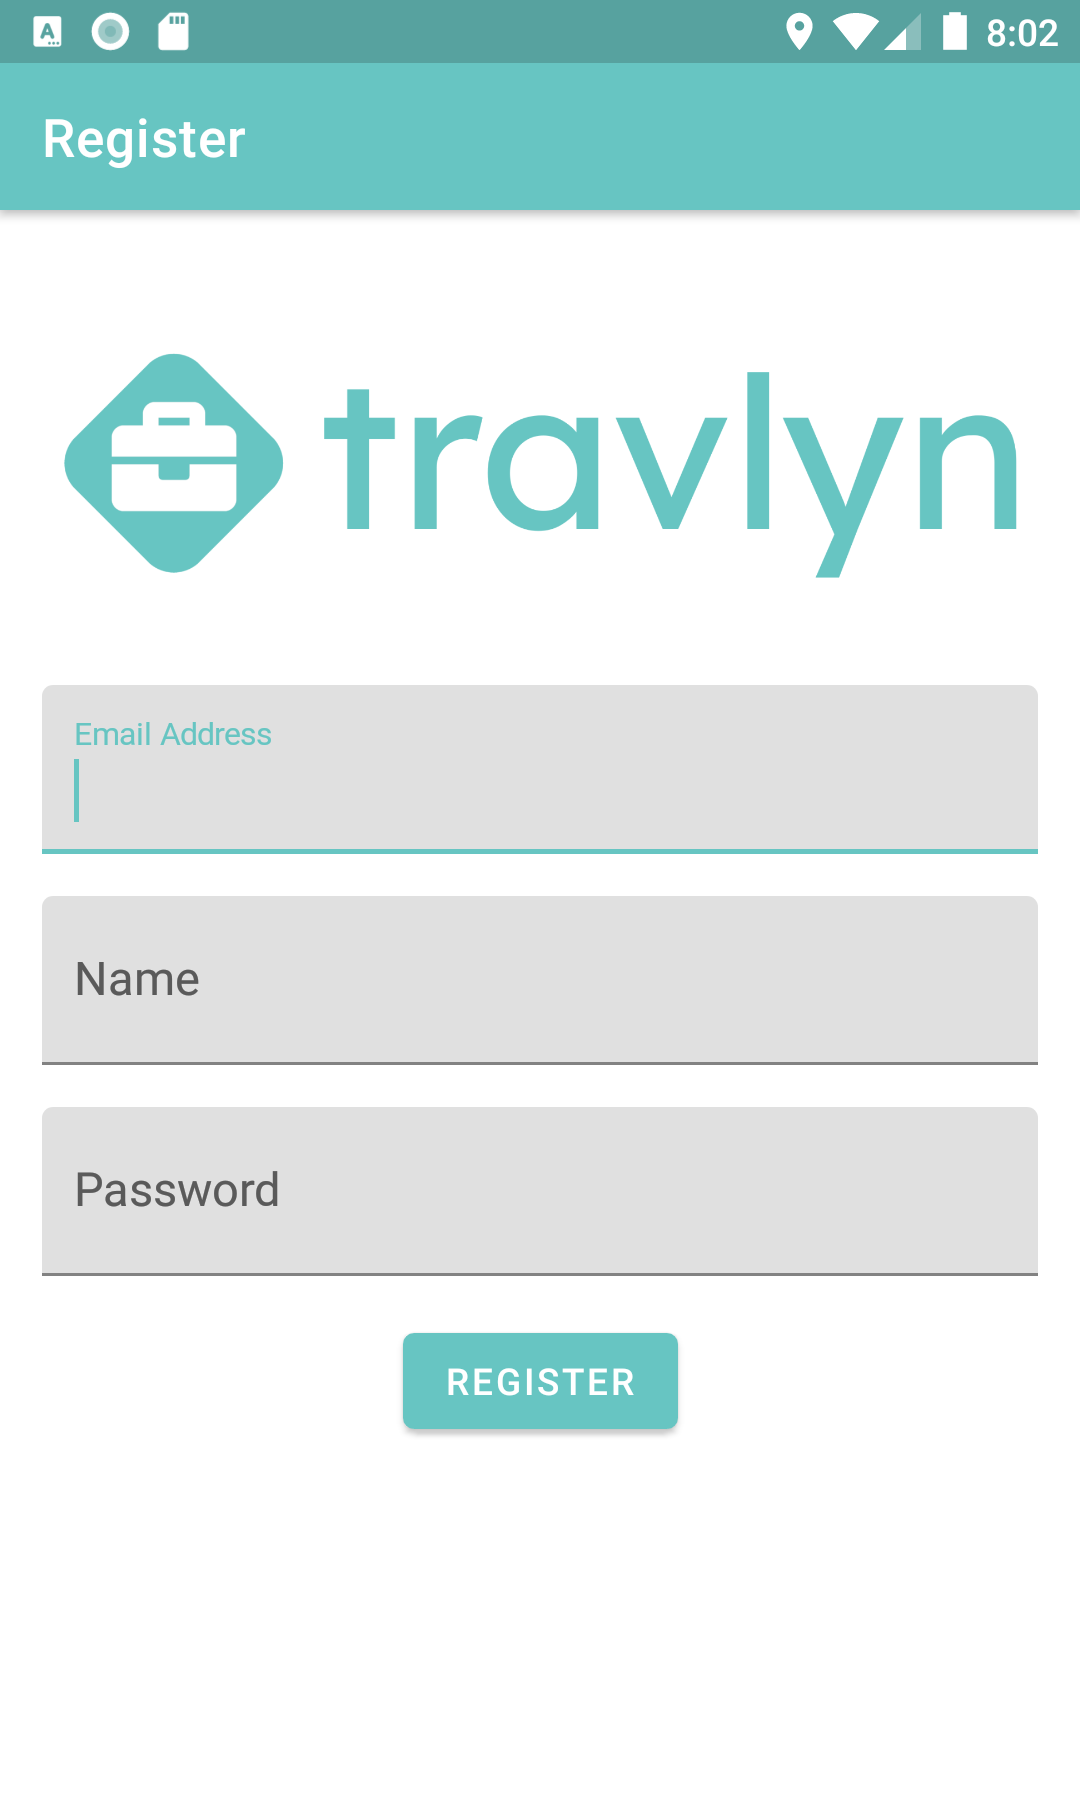
\includegraphics[width=0.32\textwidth]{images/travlyn-screenshot-register.png}
		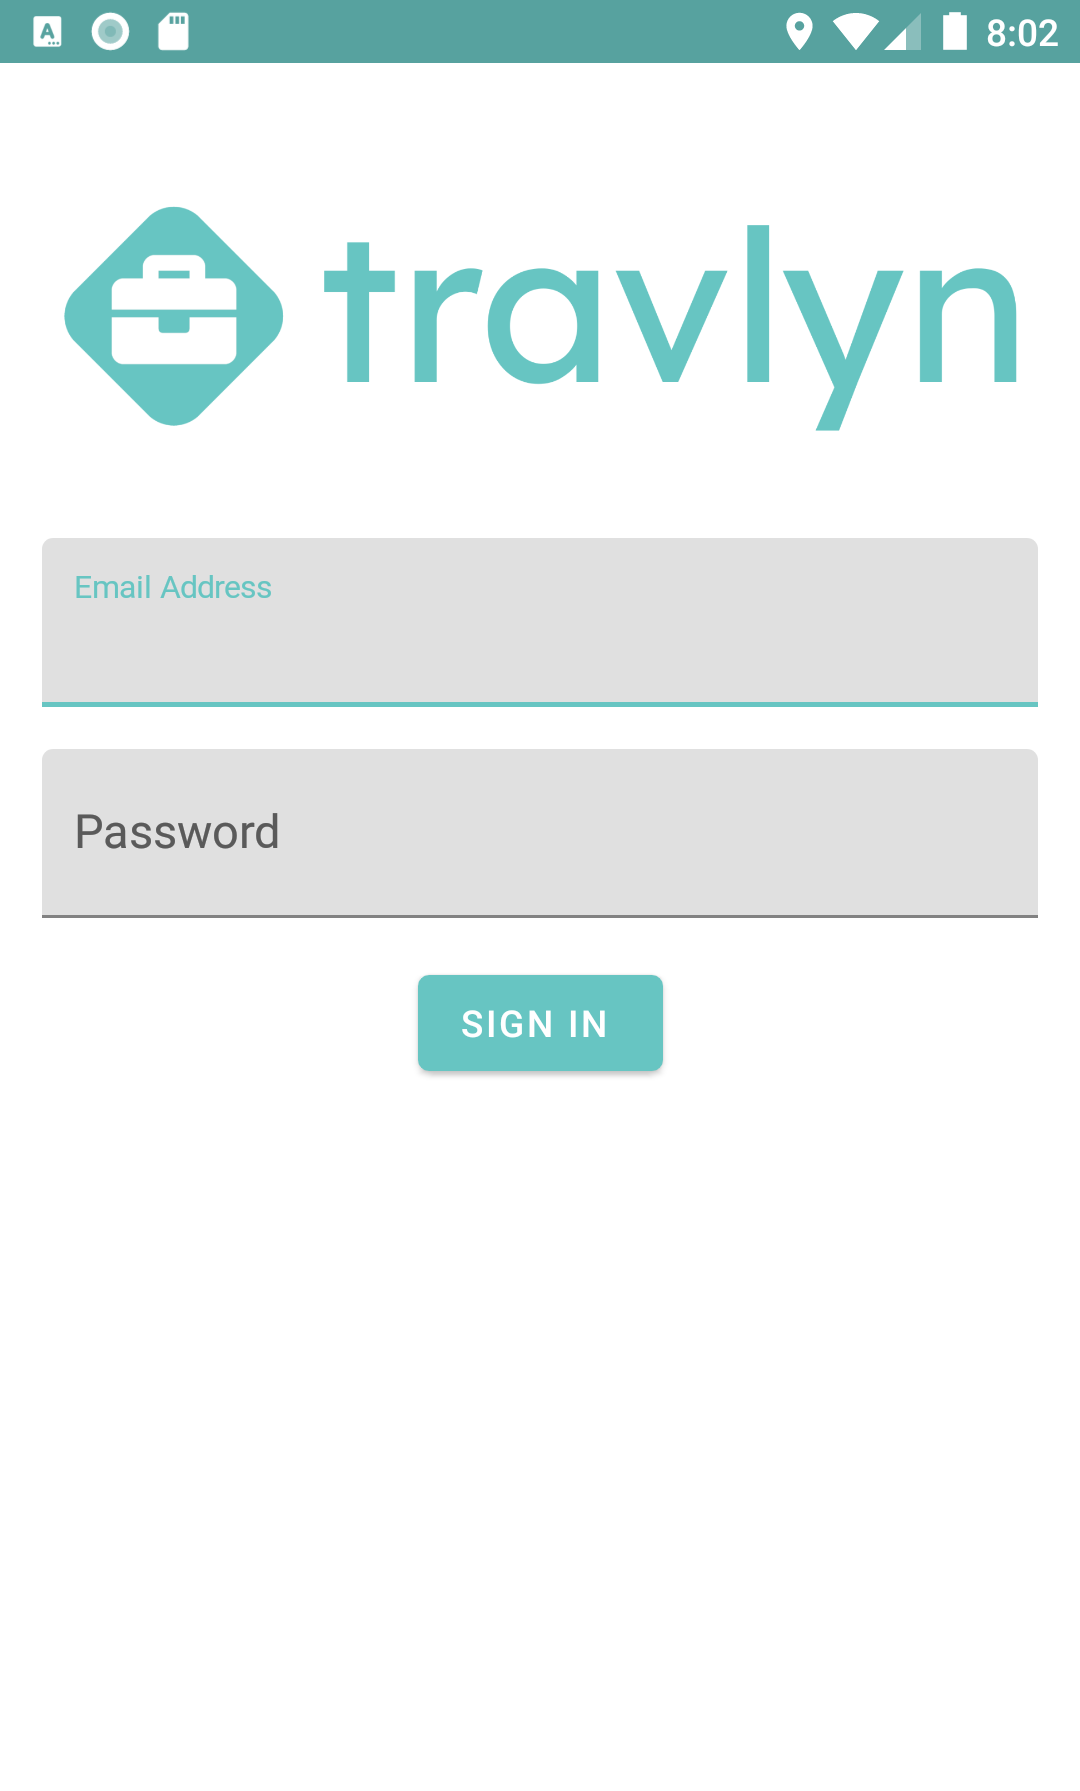
\includegraphics[width=0.32\textwidth]{images/travlyn-screenshot-login.png}
		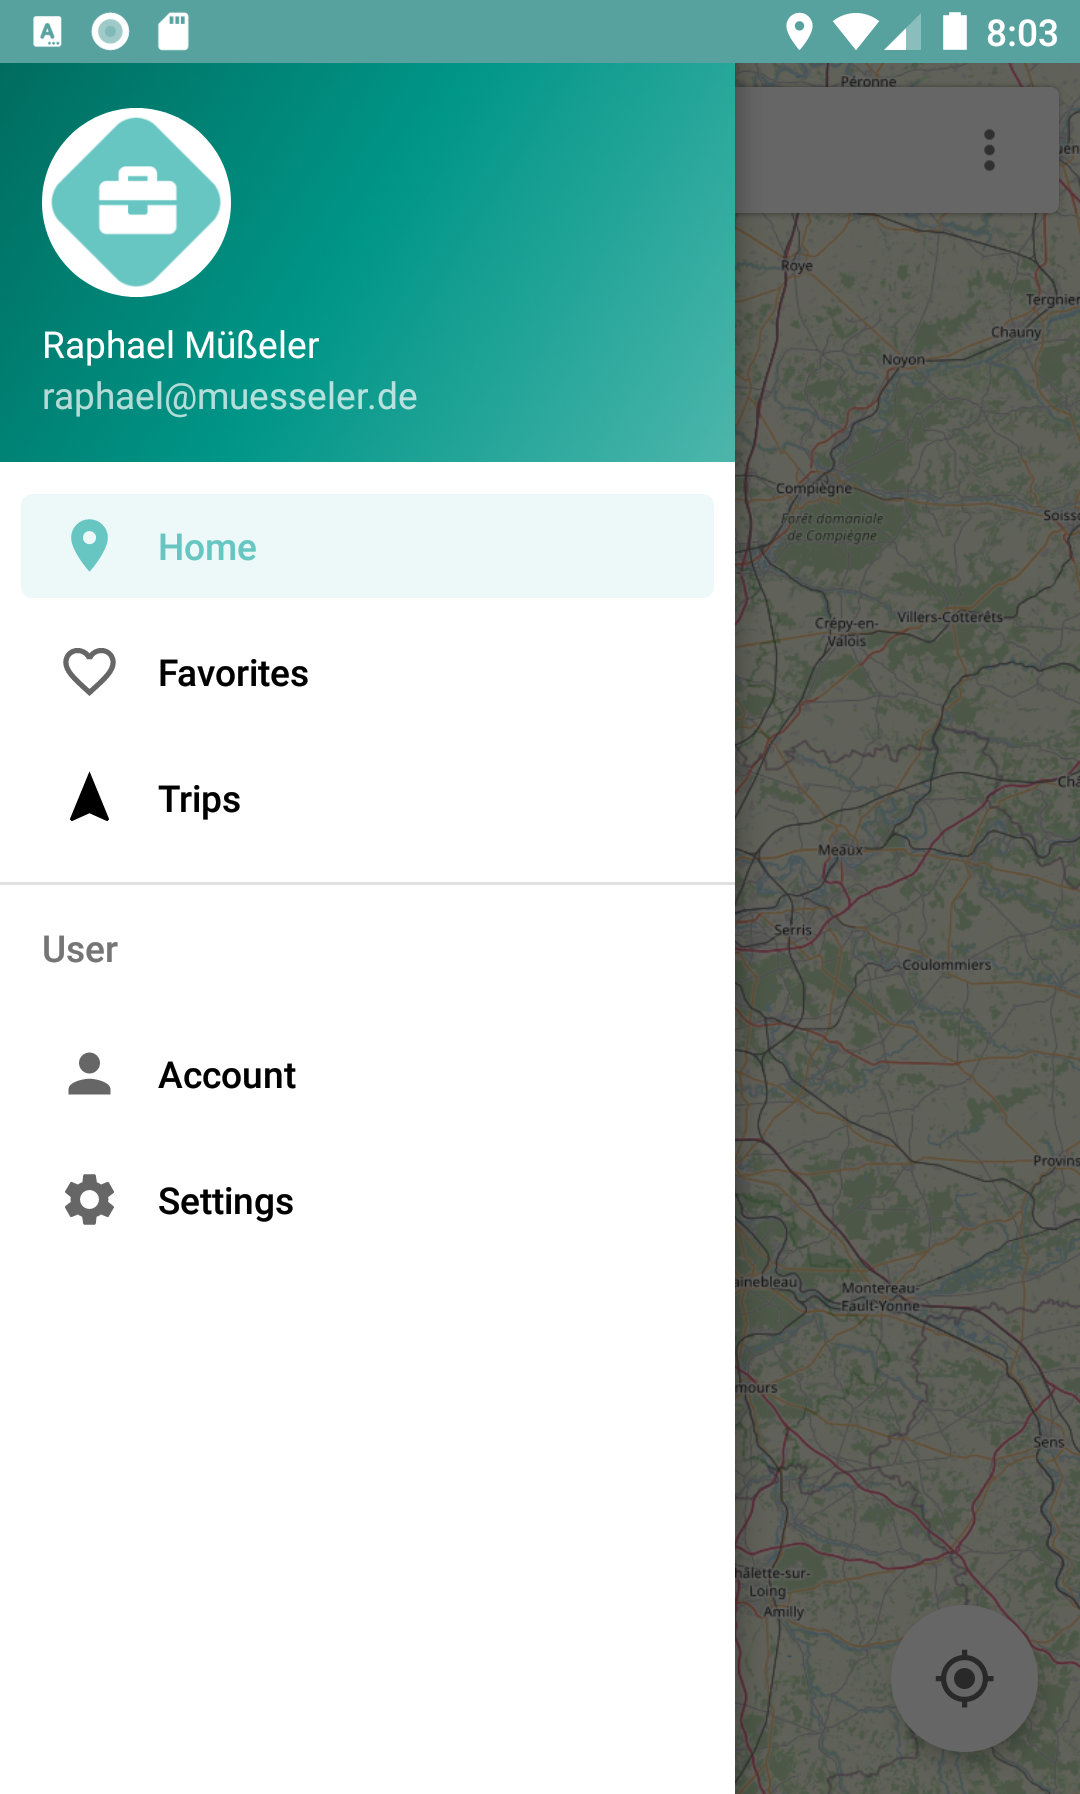
\includegraphics[width=0.32\textwidth]{images/travlyn-screenshot-side-navigation.png}
		\caption{User Management in der \textit{Travlyn} Applikation}
		\label{fig:ui_usermanagement}
	\end{figure}

	\newpage

 
	\item \textbf{Information über Städte:} In diesem Prozess kann ein Nutzer über die verfügbare Suchleiste nach jeder beliebigen Stadt auf der Welt suchen und erhält eine Beschreibung dieses Ortes. Falls es Sehenswürdigkeiten in direkter Nähe dieser Stadt gibt werden diese angezeigt und können in einer Detailliste mit ihren Metainformationen betrachtet werden. Außerdem werden ihm direkt die verfügbaren öffentlichen Trips angezeigt, welche für ihn ausführbar sind. Damit kann sich der Nutzer einen sehr vollständigen Eindruck einer Stadt verschaffen, welcher als Entscheidungsgrundlage für eine Reise dienen kann. Siehe \autoref{fig:ui_city_information}.
	
	\begin{figure}[ht!]
		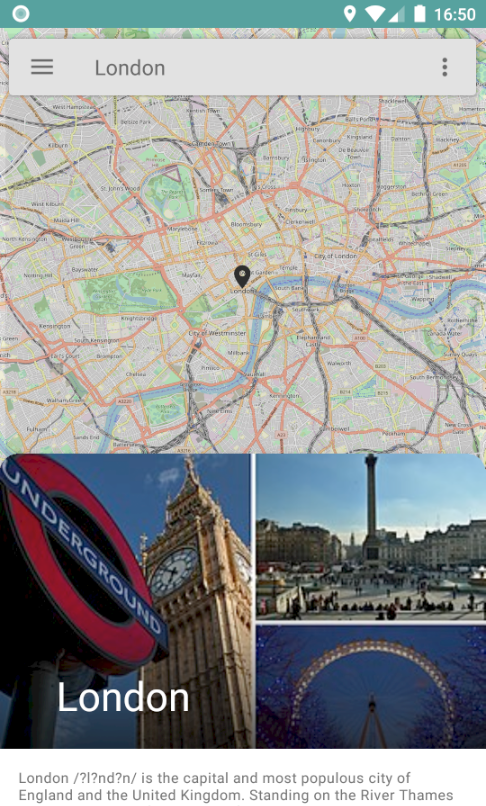
\includegraphics[width=0.32\textwidth]{images/travlyn-screenshot-search-result.png}
		
\includegraphics[width=0.32\textwidth]{images/travlyn-screenshot-city-detail.png}
		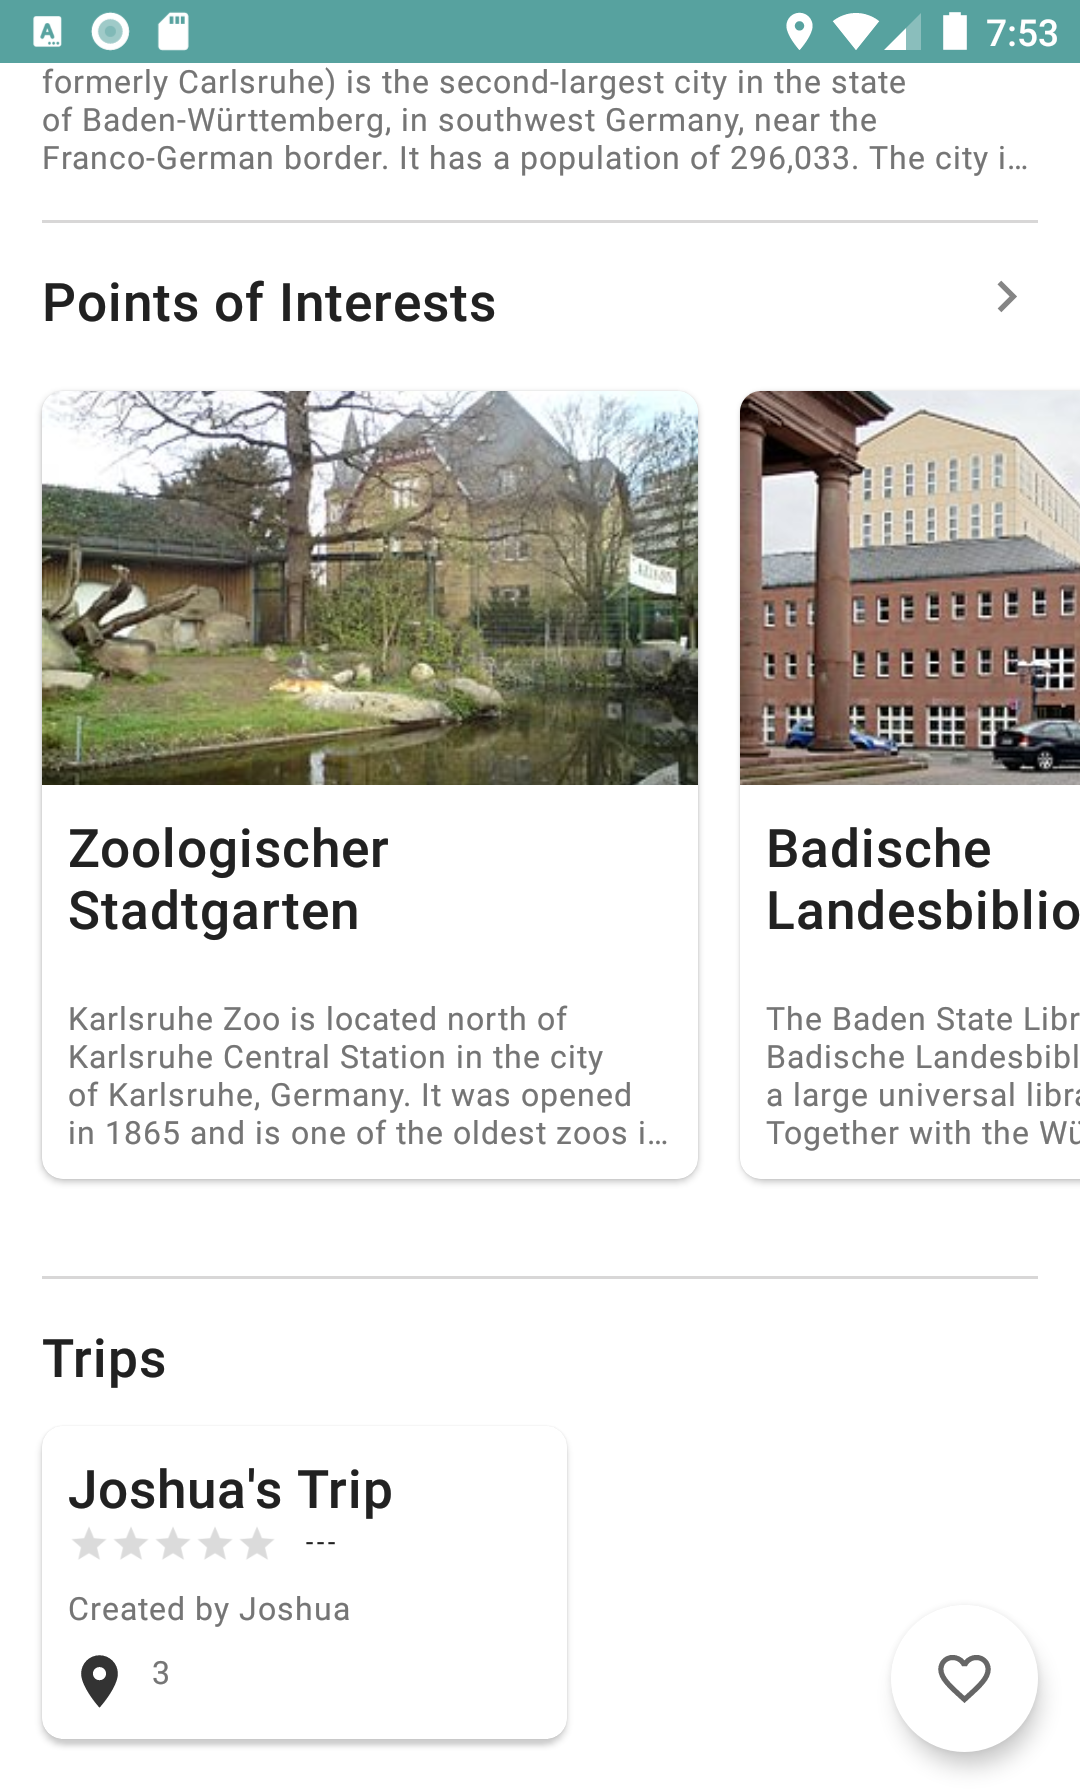
\includegraphics[width=0.32\textwidth]{images/travlyn-screenshot-city-detail-trips.png}
		\caption{Informationsangebot für eine gesuchte Stadt, in diesem Fall Karlsruhe}
		\label{fig:ui_city_information}
	\end{figure}


	\item \textbf{Trip Erstellung:} Ist eine konkrete Reise geplant, kann der Nutzer in der App einen Trip erstellen, welcher seine ausgewählten Sehenswürdigkeiten enthält und damit genau an den Umfang und Aufwand angepasst werden kann, den sich der Nutzer vorstellt. Es stehen ausnahmslos alle Ort und Kombinationen von Orten zur Verfügung. Nach der Auswahl und dem festlegen einiger Metainformationen ist der Trip direkt bereit zur Ausführung. Siehe \autoref{fig:ui_trip_creation}.
	
	\begin{figure}[ht!]
		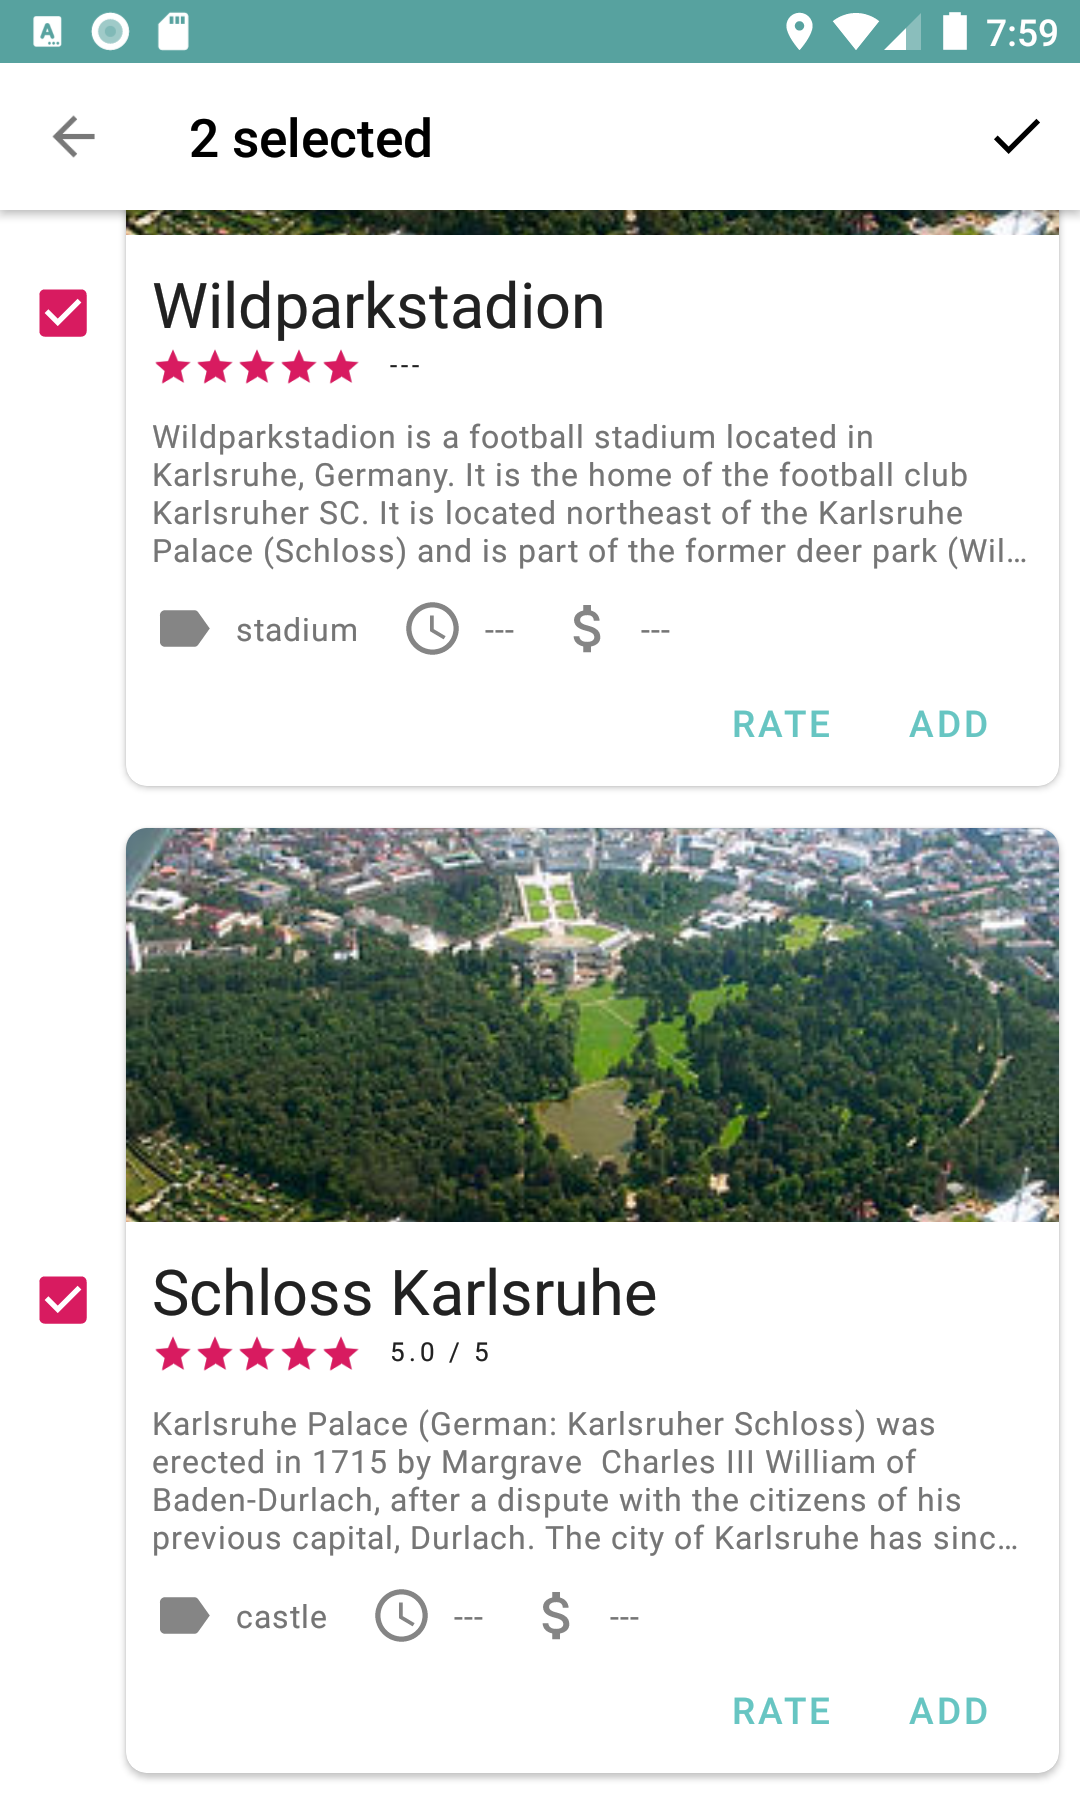
\includegraphics[width=0.32\textwidth]{images/travlyn-screenshot-stops-detail-selection.png}
		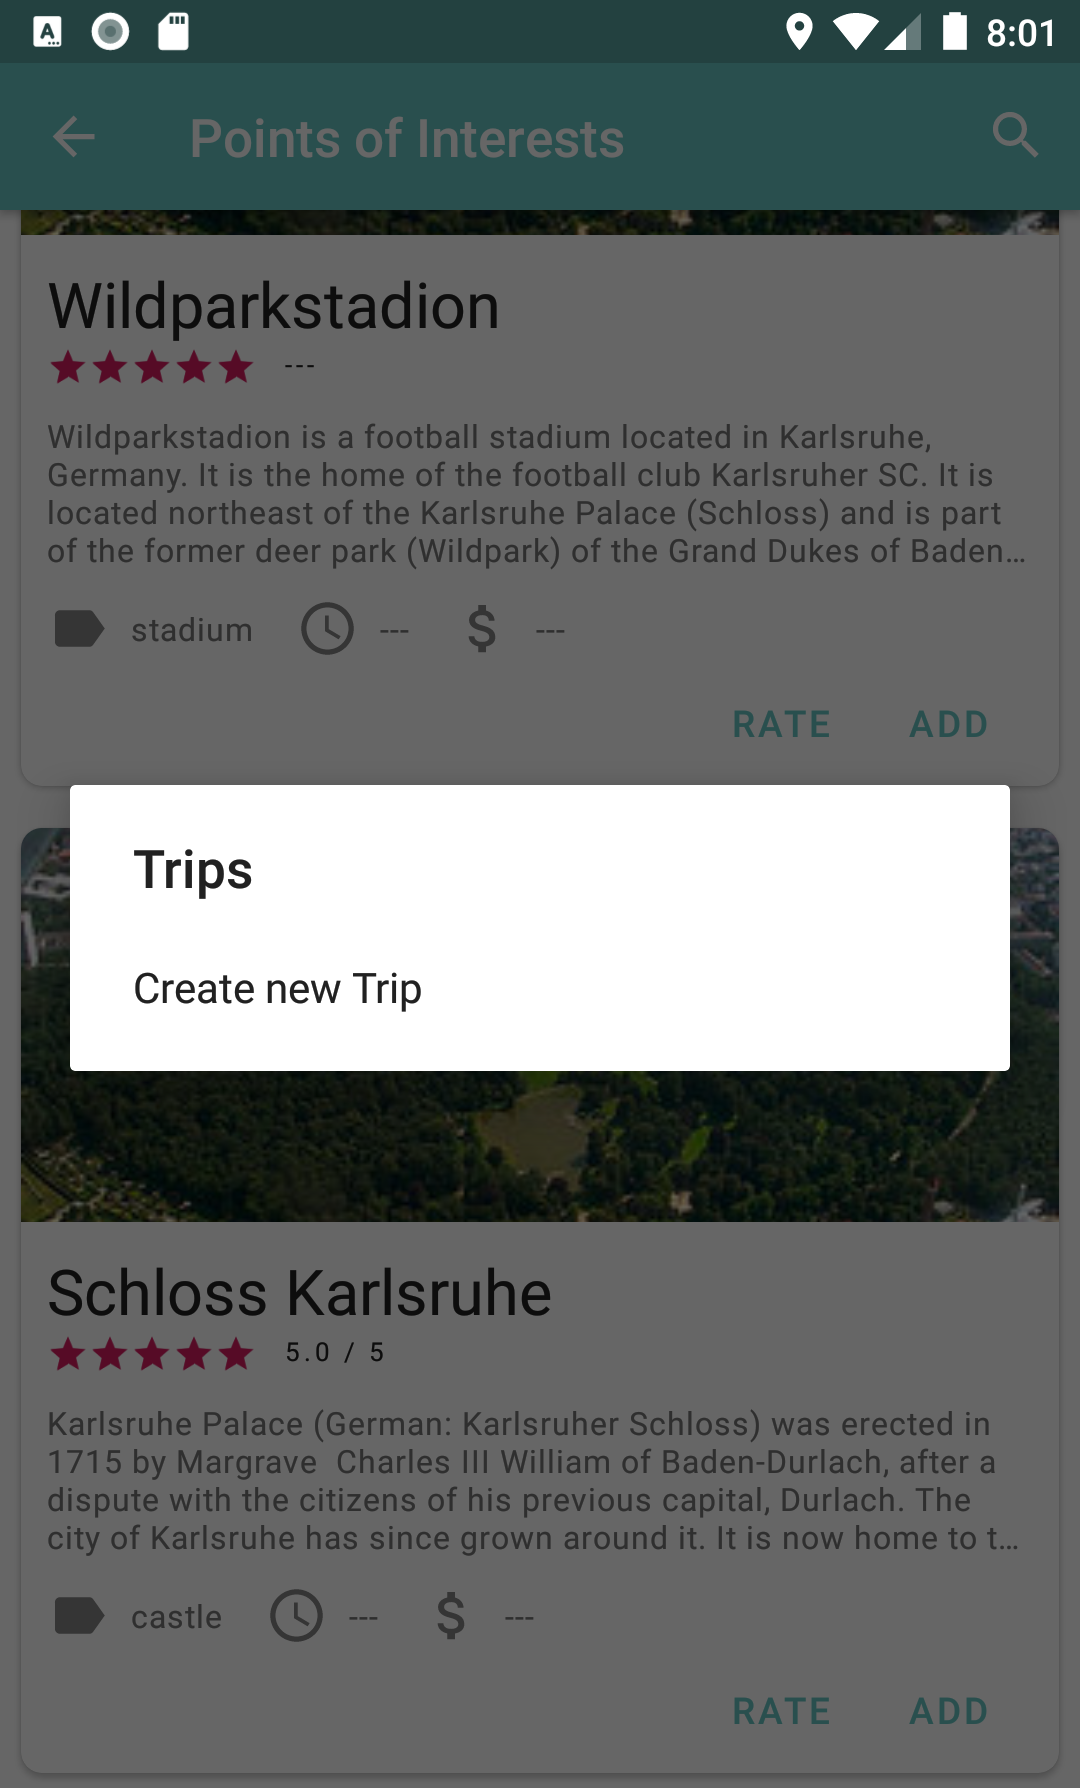
\includegraphics[width=0.32\textwidth]{images/travlyn-screenshot-stops-detail-selection-dialog.png}
		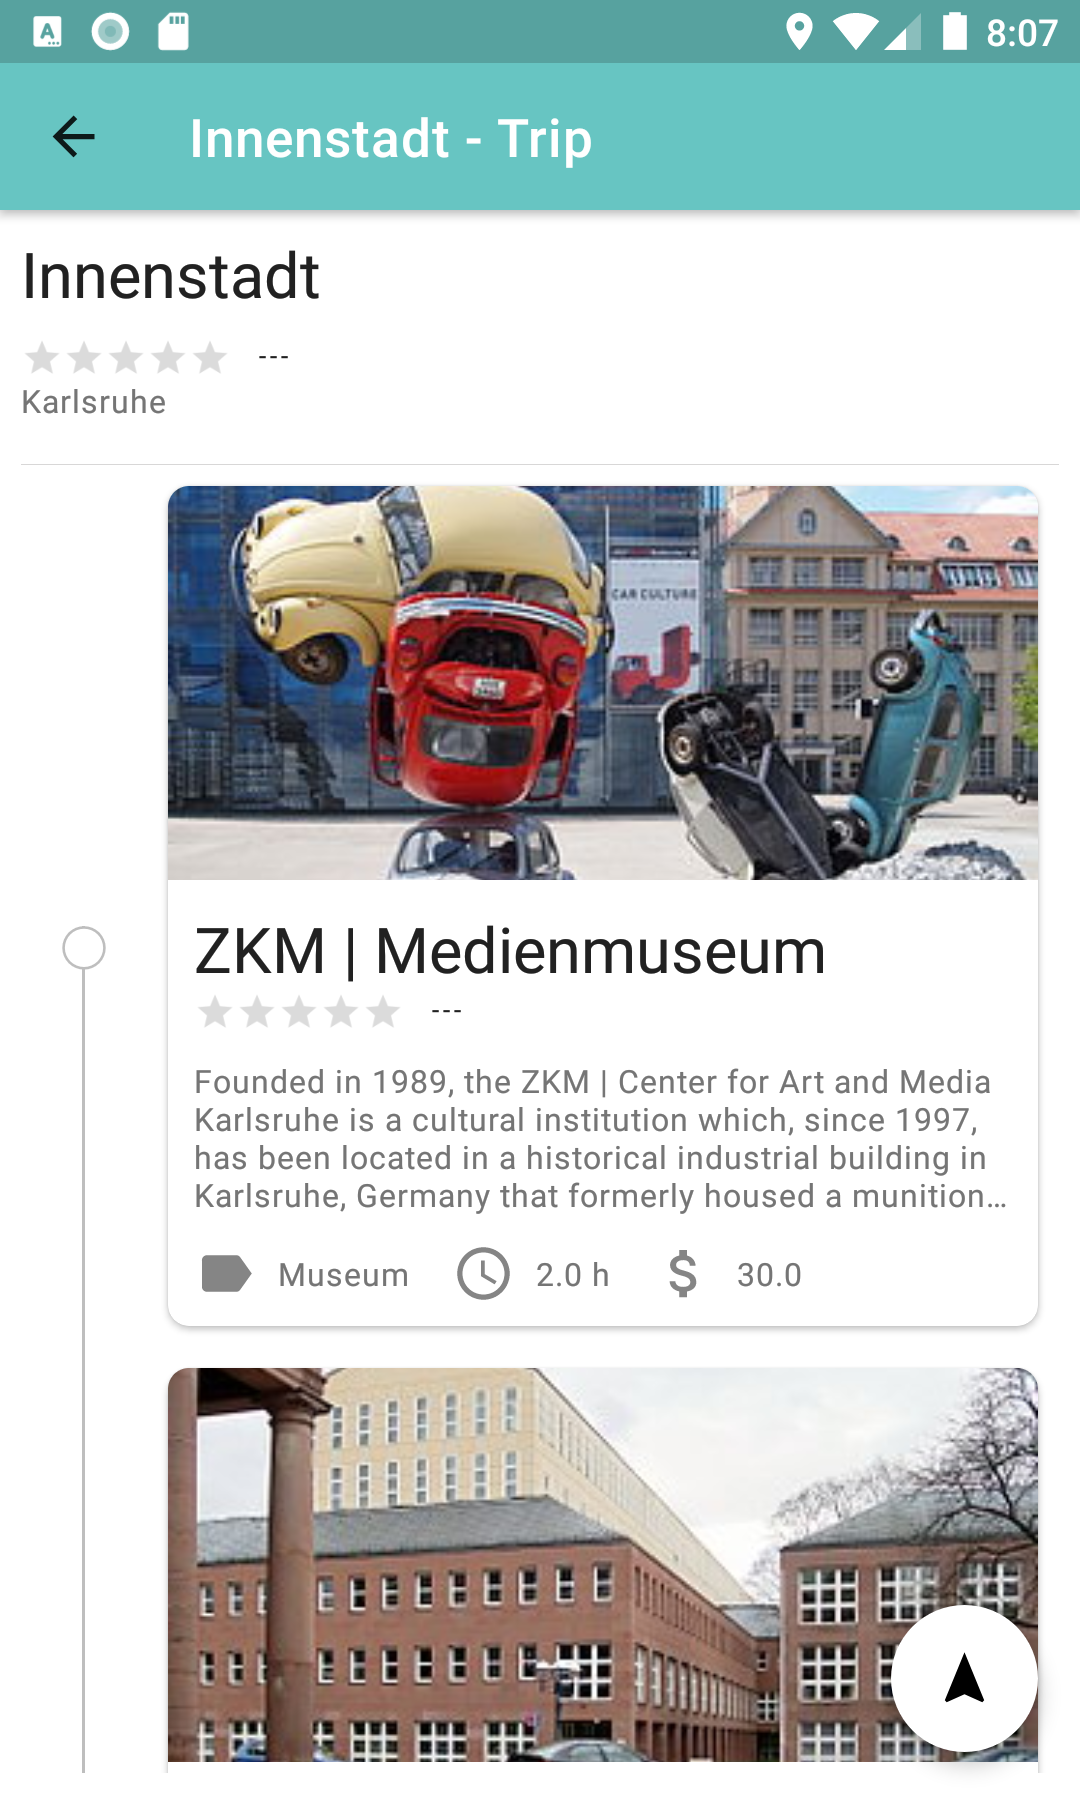
\includegraphics[width=0.32\textwidth]{images/travlyn-screenshot-trip-detail.png}
		\caption{Erstellung eines Trips anhand der bereitgestellten Stops}
		\label{fig:ui_trip_creation}
	\end{figure}

	\newpage
	
	\item \textbf{Trip Ausführung:} Am Urlaubsort angekommen können Trips ausgeführt werden. Es ist irrelevant, ob der auszuführende Trip ein eigener Trip ist oder ein öffentlicher Trip eines anderen Nutzers. Die Ausführung beinhaltet eine Navigation durch die Stadt, Informationen zu den einzelnen besuchten Sehenswürdigkeiten und die Möglichkeit die festgelegte Route zu verlassen und von der App trotzdem zum nächsten Stop geführt zu werden. Damit hat der Nutzer volle Flexibilität und eine sehr persönliche Reiseerfahrung.
	
	\begin{figure}[ht!]
		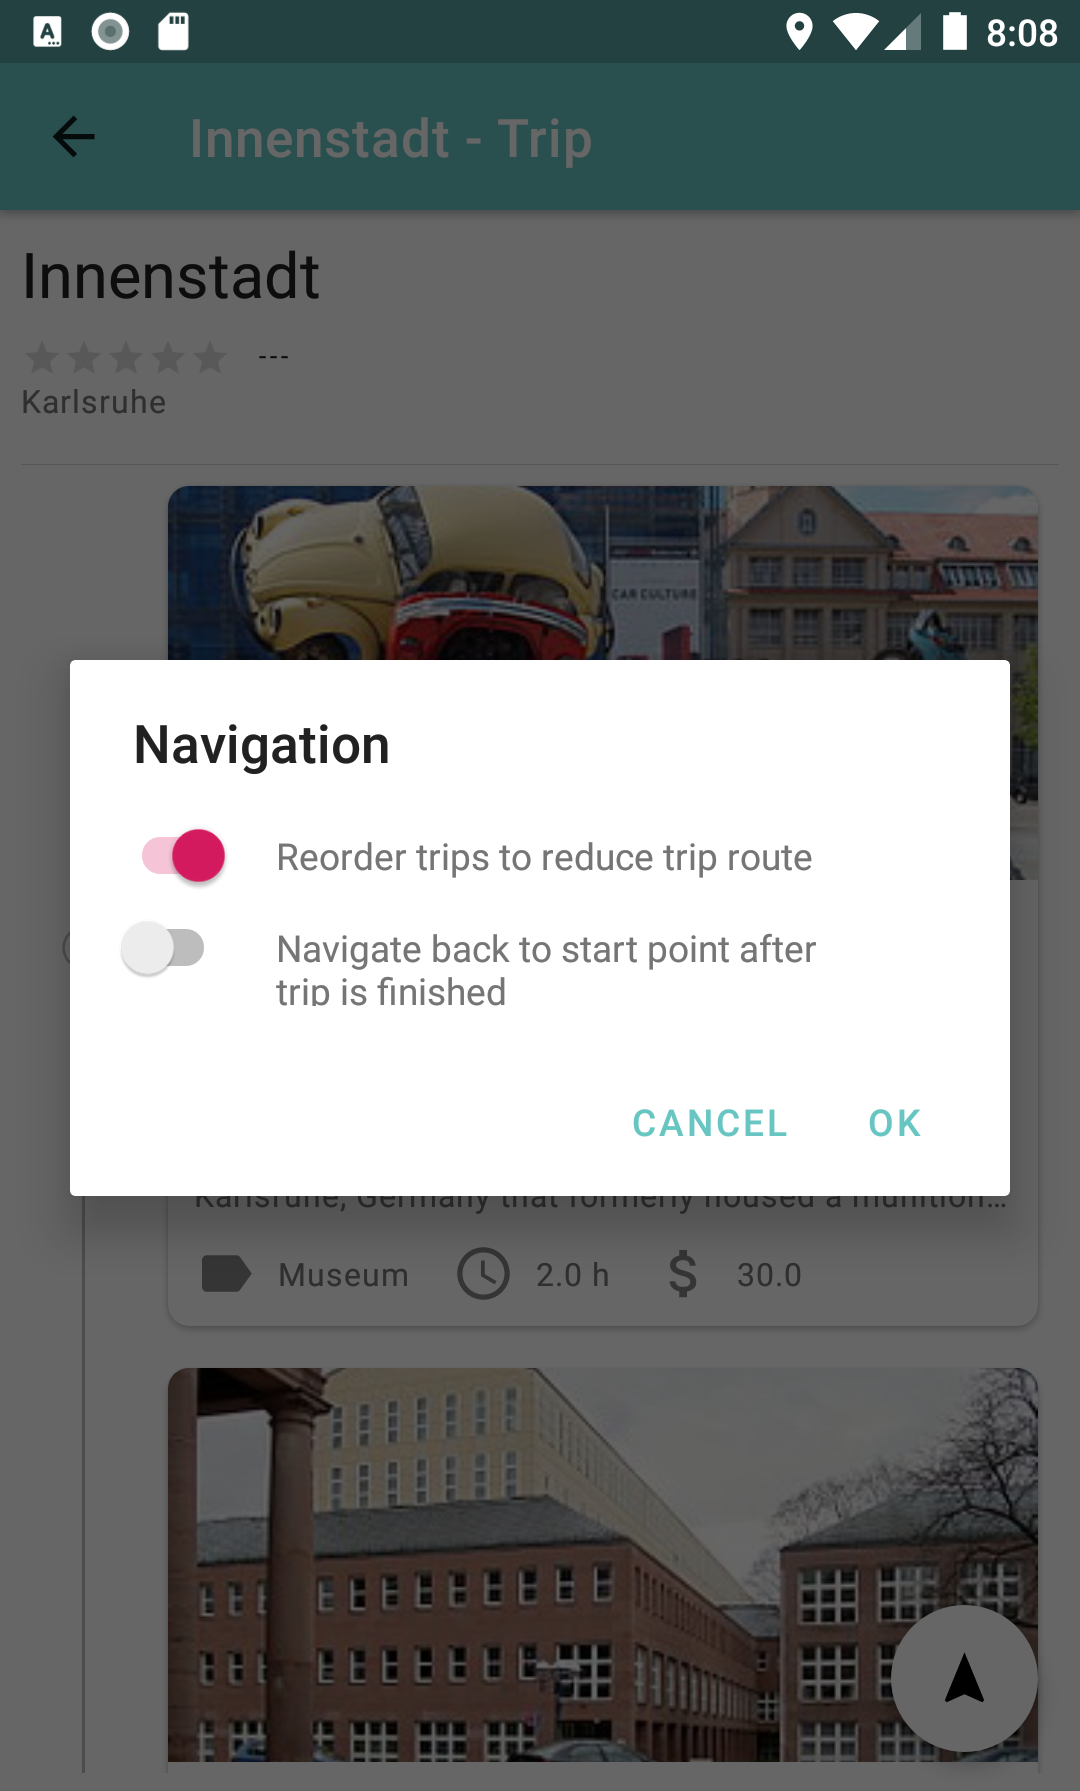
\includegraphics[width=0.32\textwidth]{images/travlyn-screenshot-start-navigation-dialog.png}
		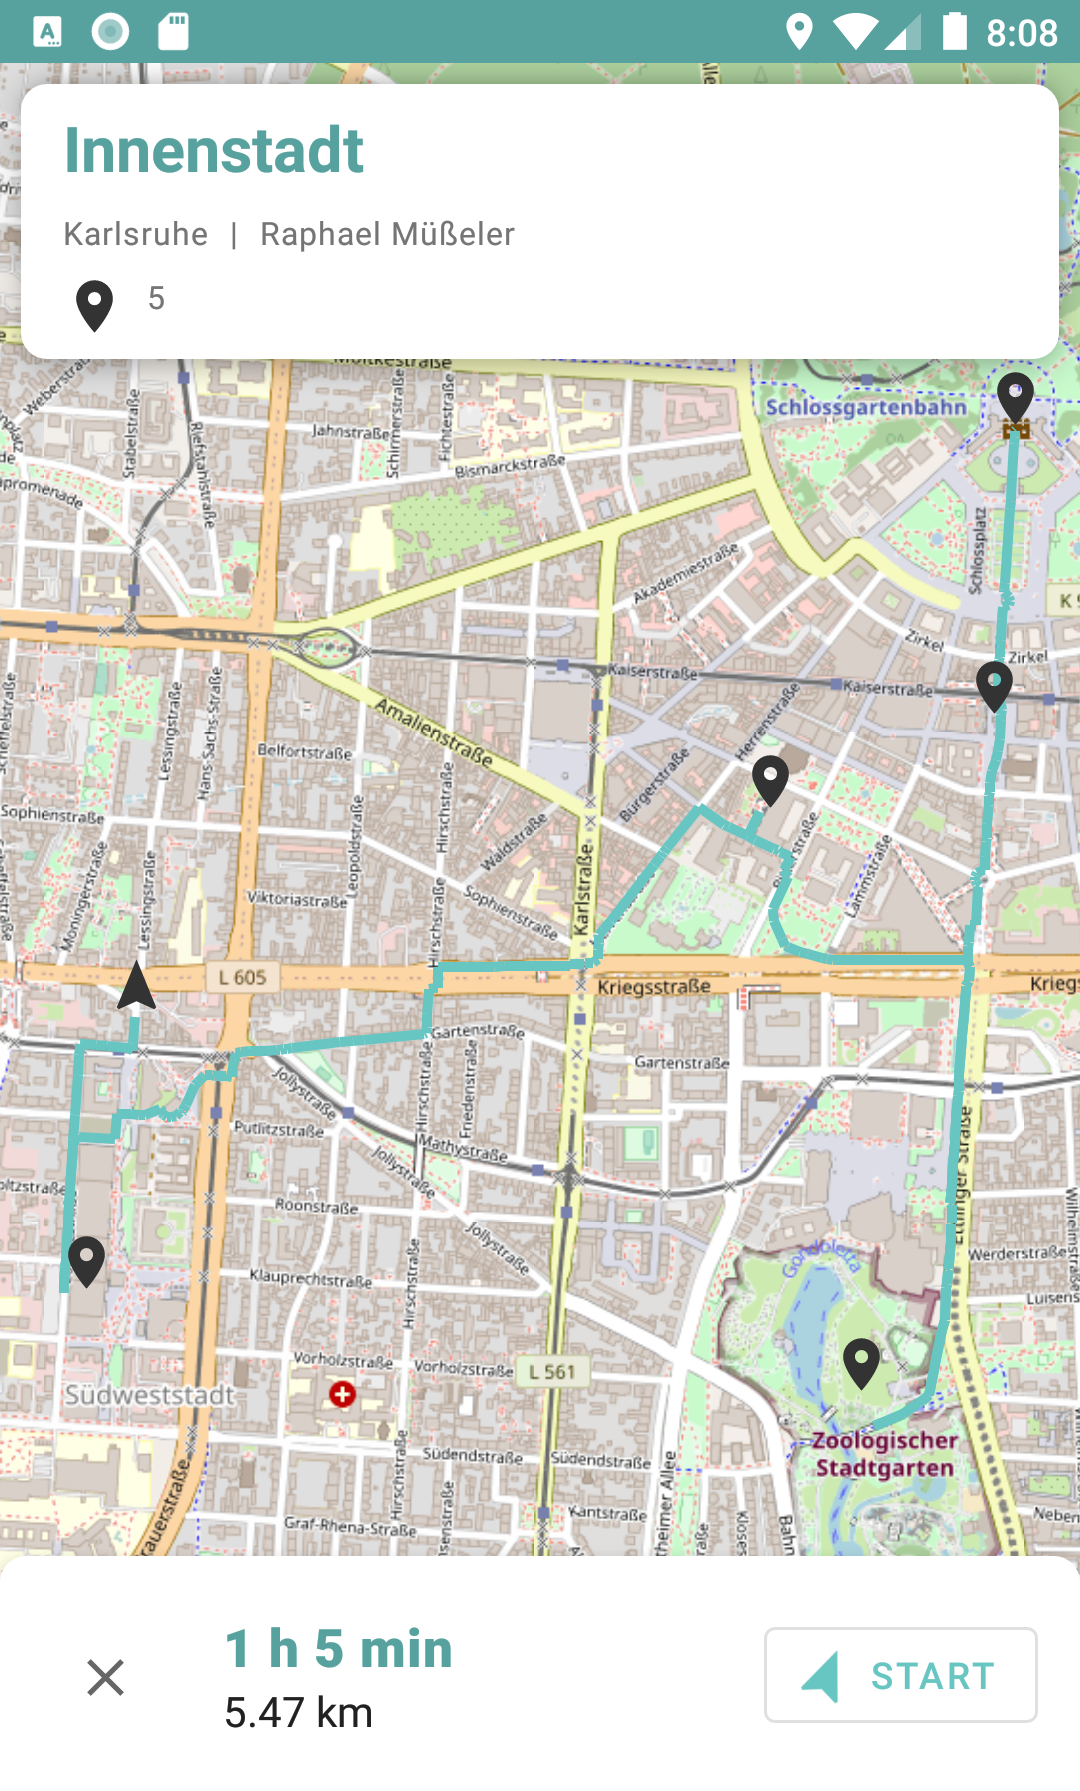
\includegraphics[width=0.32\textwidth]{images/travlyn-screenshot-navigation-overview.png}
		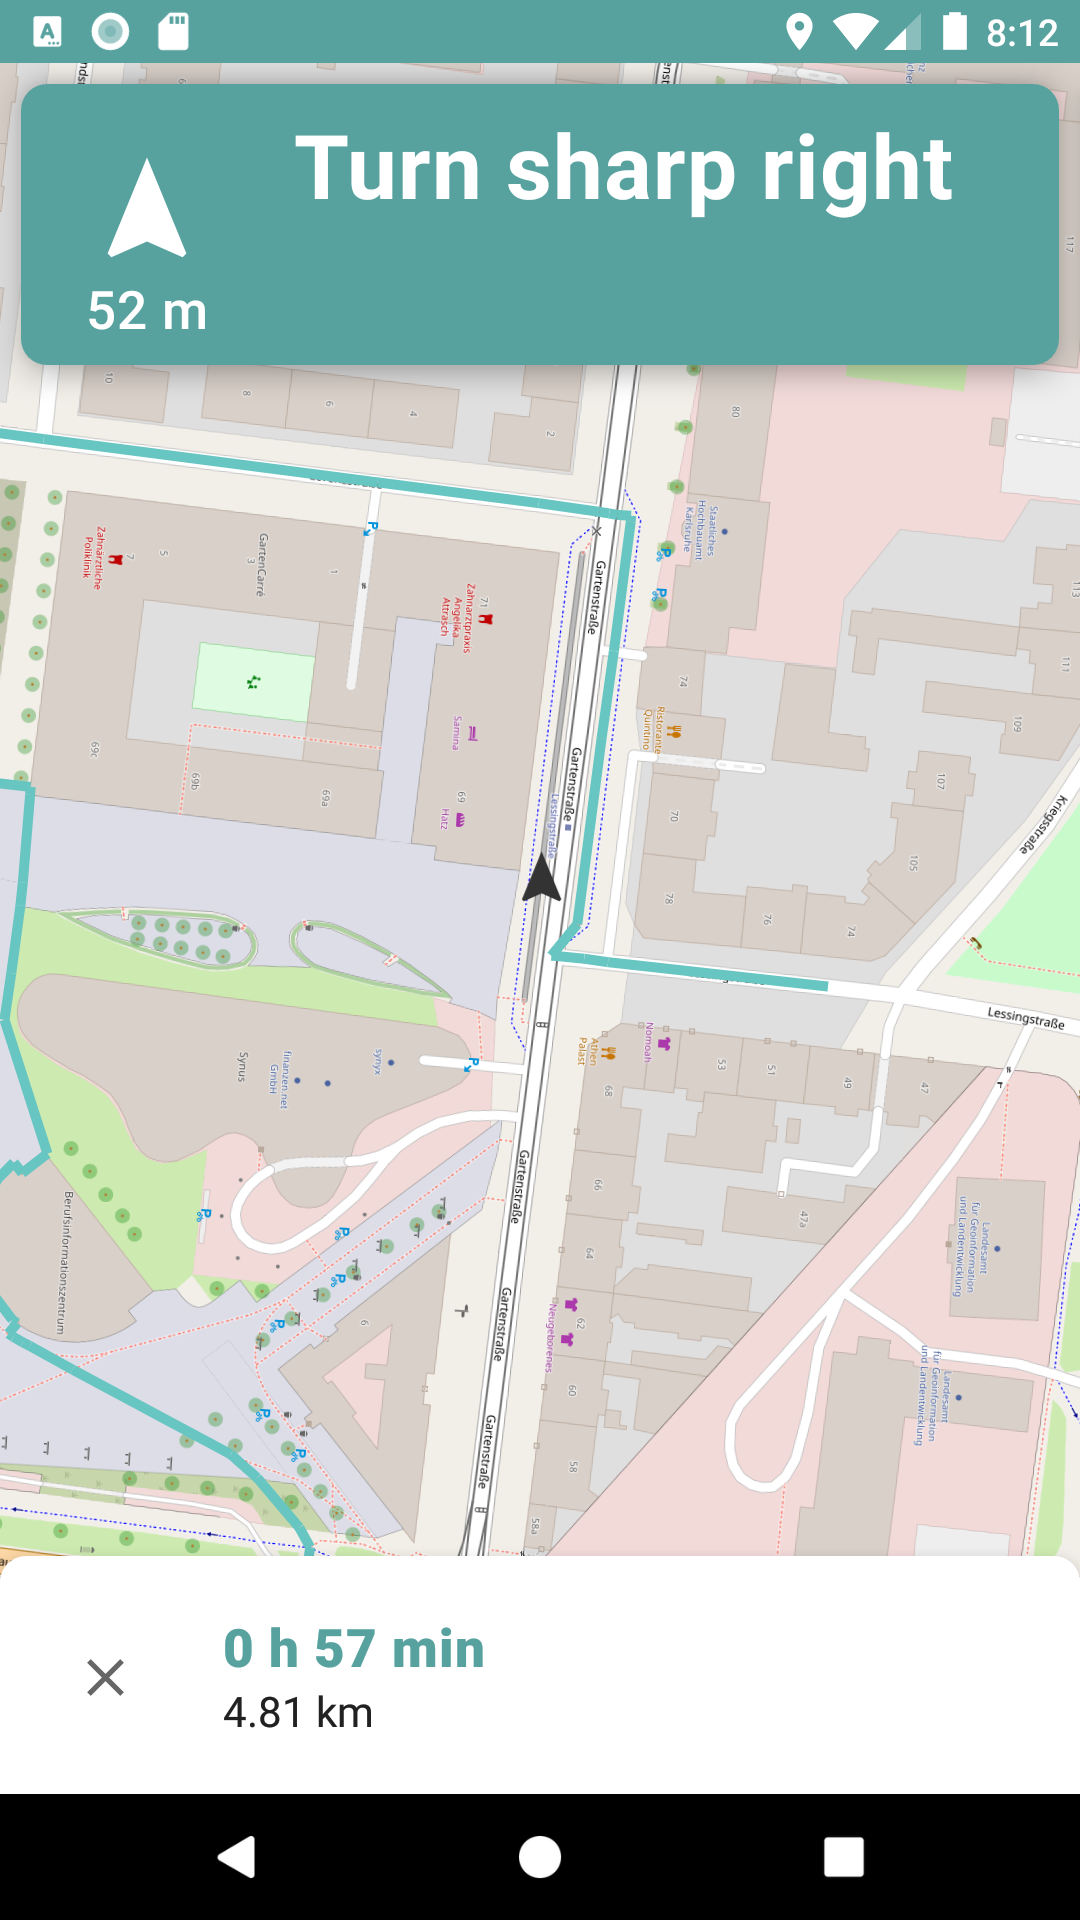
\includegraphics[width=0.32\textwidth]{images/travlyn-screenshot-navigation.png}
		\caption{Ausführung eines vorher erstellen Trips mit der \textit{Travlyn} App}
		\label{fig:ui_trip_execution}
	\end{figure}
    
\end{itemize}

Vergleicht man die beschriebenen Prozesse mit \autoref{fig:UCD} können alle Use Cases abgedeckt werden außer \textit{Share Trip}. Dieser Use Case war von Anfang an eher niedrig priorisiert und es hat sich im Verlauf der Arbeit herausgestellt, dass der Aufwand in keinem Verhältnis zum Ergebnis und somit wurde dieser Use Case nicht umgesetzt. Außerdem ist der Punkt \textit{Use API for custom purposes} und \textit{Get Trip Meta Data} nur als teilweise vollständig zu betrachten: Die erstelle API ist öffentlich zugänglich und kann mit einem API Schlüssel genutzt werden, allerdings gibt es keine automatische Generierung des Schlüssels. Diese Funktionalität ist für den Kern der \textit{Travlyn} App nicht von Bedeutung und wurde deshalb hinten angestellt.

\vspace{0.25cm}

Betrachtet man die API Use Cases als halb erfüllt, ergibt sich für die 10 übergeordneten Use Cases ein Erfüllungsgrad von 80\%, was als Erfolg gewertet werden kann, da ein Großteil der Nutzerprofile vollständig angeboten werden kann.

\section{Nicht-funktionale Anforderungen}
Neben den beschriebenen funktionalen Anforderungen wurden in \autoref{sec:anforderungen} auch nicht-funktionale Anforderungen gestellt, welche über die reine Funktionalität der App hinausgehen. Diese werden im Folgenden aufgegriffen und das entstandene Ergebnis gegen die Ziele validiert.

	\subsection{Benutzbarkeit}
	Als erste Anforderung wurde eine gute Benutzbarkeit und ein ansprechende Nutzungserfahrung gefordert, da die App auf mobilen Geräten mit kleinem Bildschirm und in Situationen genutzt wird bei denen die Konzentration eher auf der erlebten Reise und nicht auf der Bedienung der App liegen sollte und Schwierigkeiten mit der App die Erfahrung beeinträchtigen würden.
	
	\vspace{0.25cm}
	
	Zur Validierung dieses Ziels gibt es sehr viele Verschiedene Methoden, die unterschiedliche Vorteile und Herausforderungen bieten. Diese Methoden reichen von \textit{Lautem Denken}, über \textit{Konstruktive Interaktion} bis zu \textit{Usability Kiosks} \cite{Nielsen.20091993}. All diese Methoden liefern Usability-Daten die zum einen durch die Auswertung der Äußerungen der Nutzer und zum anderen durch verschiedene Metriken wie z.B. die benötigte Zeit für eine Aktion, die Anzahl der begangenen Fehler oder die Anzahl der ungenutzt gebliebenen Features interpretiert werden. Es gibt feste Methoden zum planen und durchführen dieser Tests.
	
	\vspace{0.25cm}
	
	Auf Grund der aktuellen Situation, die durch das COVID-19 Virus geprägt ist und dem engen Zeitplan für diese Arbeit, können leider viele der von \cite{Nielsen.20091993} vorgestellten Methoden nicht ausgeführt werden, da ein direkter Kontakt zu den Testnutzer erforderlich wäre. Somit ist es notwendig ein kontaktloses und vom Umfang angemessenes Verfahren zu finden, welches einen wissenschaftlich begründeten Überblick über die erreichte Usability bietet.
	
	Schlussendlich viel die Entscheidung auf die \ac{SUS} \cite{Brooke.1996}. Diese Skala wurde von John Brooke entwickelt und konzentriert sich auf einen schnellen und kostengüstigen Test der Usability. Ursprünglich entstand diese Umfrage im Bereich der Industrie, in der oft schnelle und grundlegende Usability-Bewertungen benötigt werden, ohne dass viele Testpersonen über Stunden befragt werden müssen oder komplizierte Auswertungen durchgeführt werden müssen. Trotz den beschriebenen Abstrichen hat sich diese Methode in der Industrie durchgesetzt und ist weit etabliert \cite{MatthiasRauer.11.April}. Dieses Verfahren stellt einen Usability-Wert durch eine Umfrage fest, die zehn Fragen beinhaltet. Diese werden von Testpersonen beantwortet, die vorher die Möglichkeit hatten das betreffende System zu testen, aber bevor Diskussionen mit anderen Testpersonen stattfinden. Die Antworten sollen intuitiv und ohne Nachdenken gegeben werden \cite{Brooke.1996}. Die Fragen bestehen aus grundlegenden Bewertungsfragen in denen Aussagen wie z.B:
	
	\begin{itemize}
		\item \enquote{Ich kann mir sehr gut vorstellen, das System regelmäßig zu nutzen.}
		\item \enquote{Ich empfinde das System als einfach zu nutzen.}
	\end{itemize}

bewertet werden sollen (restliche Fragen siehe \cite{Brooke.1996}). Hierfür steht eine Likert-Skala \cite{Joshi.2015} zur Verfügung, die fünf bis sieben Auswahlmöglichkeiten von \enquote{Starke Zustimmung} bis \enquote{Überhaupt keine Zustimmung} enthält.

\vspace{0.25cm}

Nach der Durchführung der Umfrage werden alle Ergebnisse anhand eines fest vorgegebenem Verfahren verrechnet: Für einen Teil der Fragen gilt die abgegebene Punktzahl der Likert-Skala minus eins und für den anderen Teil fünf minus den abgegeben Punktwert. Nach der Summation aller Werte und dem Multiplizieren mit der Konstante 2.5 ergibt sich ein Ergebniswert zwischen 0 und 100, welcher die Usability widerspiegelt und vergleichbar macht.

\vspace{0.25cm}

Da die Durchführung der Befragung sehr einfach alleine online und ohne weitere Einflussnahme der Tester/Entwickler durchgeführt werden kann und trotzdem ein wissenschaftlich anerkanntes Ergebnis liefert wurde für \textit{Travlyn} ein Test mit der \acs{SUS} durchgeführt. Im Folgenden wird die konkrete Durchführung dieses Verfahrens aufgezeigt.    
	
		\subsubsection{Aufbau}
		Zur Vorbereitung des Experiments wurde ein Server mit dem \textit{Travlyn}-Backend aufgesetzt und die App als \acs{APK}-Datei erstellt. Durch den Jenkins-Buildserver war diese automatische Erstellung sehr einfach und schnell. Des Weiteren wurden geeignete Testpersonen ausgesucht: Da die Zielgruppe der Applikation jeden umfasst der gerne reist, kamen viele Personen aus dem Umfeld des Entwicklungsteams infrage. Ausgewählt wurde schließlich eine Gruppe von TODO Testpersonen, die einen Durchschnitt über das Alter bilden (von 14 bis Ende 50 TODO) und alle Nutzergruppen von praktisch keiner Technikerfahrung bis ausgiebiger täglicher Technikerfahrung abdecken. Für die Online Befragung wurde das zu Google gehörende Tool \textit{Google Forms} verwendet \cite{Google.2020}.
		
		\subsubsection{Ablauf}
		Nach der Auswahl und Erstellung aller oben beschrieben Artefakte wurde eine Mail mit der Applikationsdatei und dem Link zur Umfrage an alle Testpersonen verschickt. Alle Testpersonen sollen die Applikation selbständig installieren und nach Belieben ausprobieren. Im direkten Anschluss soll der bereitgestellte Link genutzt werden, um die Onlineumfrage auszufüllen. Bei technischen Problemen standen die Entwickler über digitale Kanäle zur Hilfe bereit.
		Durch die Nutzung des Google Tools läuft die Zusammenstellung der Ergebnisse automatisch ab und kann gesammelt abgerufen werden.  
		\subsubsection{Ergebnis}
		Die abgerufenen Ergebnisse wurden wie oben beschrieben verrechnet, pro Frage wird die durchschnittliche Antwort errechnet und entsprechen der zwei Rechenregeln ein endgültiger Wert bestimmt (Fragen 1, 3, 5, 7 und 9: Antwort minus eins; Fragen 2, 4, 6, 8 und 10: fünf minus den Antwortwert). Damit ergeben sich folgende Werte:
		
		\begin{itemize}
			\item \textbf{Frage 1:} Durchschnitt: 4.714, damit endgültiger Wert: 3.714
			\item \textbf{Frage 2:} Durchschnitt: 1.166, damit endgültiger Wert: 3.834
			\item \textbf{Frage 3:} Durchschnitt: 5.0, damit endgültiger Wert: 4.0
			\item \textbf{Frage 4:} Durchschnitt: 1.0, damit endgültiger Wert: 4.0
			\item \textbf{Frage 5:} Durchschnitt: 5.0, damit endgültiger Wert: 4.0
			\item \textbf{Frage 6:} Durchschnitt: 1.166, damit endgültiger Wert: 3.834
			\item \textbf{Frage 7:} Durchschnitt: 4.333, damit endgültiger Wert: 3.333
			\item \textbf{Frage 8:} Durchschnitt: 1.333, damit endgültiger Wert: 3.667
			\item \textbf{Frage 9:} Durchschnitt: 4.5, damit endgültiger Wert: 3.5
			\item \textbf{Frage 10:} Durchschnitt: 1.333, damit endgültiger Wert: 3.667
		\end{itemize}
	
	Zur Berechnung des Skalawerts zwischen 0 und 100 werden alle endgültigen Werte aufsummiert und mit 2,5 multipliziert:
	
	\begin{itemize}
		\item Summe: 37.8725, damit Usabilityscore: $37.8725*2.5=93.8725$
	\end{itemize}

	Der vorliegende Usabilityscore von xxx zeigt, dass ...... TODO
	
	\subsubsection{Weitere Hinweise}
	Wie in \cite{Nielsen.20091993} beschrieben gibt es im Usability-Testing einige Fallstricke und viele Methoden haben Probleme mit Zuverlässlichkeit und Validität. Somit ist nicht zwingend sichergestellt, dass diese Usability-Experimente bei wiederholter Ausführung das gleiche Ergebnis ergibt und ob das Ergebnis des Experiments wirklich die zu testende Eigenschaft widerspiegelt. Somit ist das obenstehende Ergebnis als Orientierung zu erachten und müsste durch weitere Tests, welche wir unter den aktuellen Umständen leider nicht durchführen können, validiert werden.
	
	\subsection{Sicherheit}
	Um die Sicherheit des Codes zu überprüfen wurden diverse Methoden eingesetzt, welche in \autoref{sec:QM} beschrieben wurden. Die erste ebene ist die Testebene: Es wurde Wert auf Tests gelegt, welche möglichst viele Szenarios und vor allem Fehlerfälle abdeckt, damit wird sicher gestellt, dass die einzelnen Einheiten sich im Falle einer unerwarteten Situation richtig verhalten und somit nicht angreifbar sind. Beispielsweise wird auf den entsprechenden Trip Endpoints getestet, dass ein Nutzer nur auf private Trips zugreifen kann, wenn er eingeloggt ist und einen Trip abruft, der seinem Account zugeordnet ist.
	
	\vspace{0.25cm}
	
	Neben den Tests gibt es mit SonarQube eine weitere technische Kontrollinstanz. Dieses Tool analysiert, wie in \autoref{qm.sonarqube} beschreiben, statisch den Code um nach Fehlern und vor allem Verwundbarkeiten und Bugs zu suchen. Durch diese Analyse sind während der Implementation immer wieder Konstrukte aufgefallen, welche eine Angriffsmöglichkeit dargestellt hätten. Durch die Detektion von SonarQube konnten diese Fehler allerdings behoben werden, sodass \textit{Travlyn} nun den Top zehn Sicherheitsstandards der OWASP Foundation \cite{OWASPFoundation.20200503T01:28:27.000Z} genügt. \autoref{fig:sonarqube_result} zeigt diese Top zehn Liste und dass keine entsprechende Stelle im Code gefunden wurde.
	
	\begin{figure}[ht!]
		\centering
		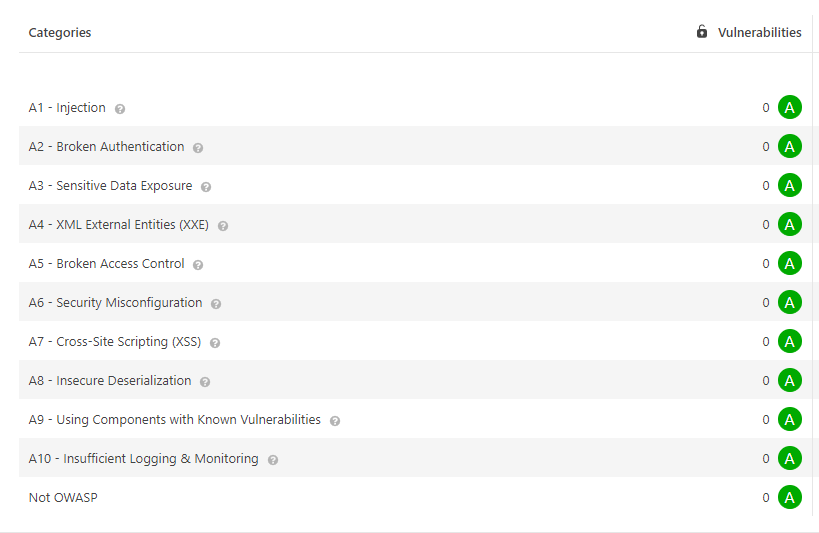
\includegraphics[width=1\textwidth]{images/Verwundbarkeiten_SonarQube.png}
		\caption{Erkannte Verwundbarkeiten durch SonarQube}
		\label{fig:sonarqube_result}
	\end{figure}

	Neben den technischen Möglichkeiten wurde der erstellte Code während der Entwicklung regelmäßig durch gemeinsame Reviews durch die Entwickler validiert. Wie in \autoref{sec:QM} beschrieben wurde jeder Pull Request vor dem Einfügen in den Master-Branch reviewed und bei entsprechenden Fehlern und Unklarheiten solange geändert, bis alle Zweifel ausgeräumt waren. Somit genügt der Code dem \enquote{Vier-Augen-Prinzip} und Fehler welche die technischen Hilfsmittel nicht aufdecken konnten wurden in diesem Prozess gefunden.
	
	\vspace{0.25cm}
	
	Somit gibt es eine ausgiebige Kontrolle des Code, welcher sicherstellt, dass keine Verwundbarkeiten vorliegen. Das Ziel eine gute Sicherheit für \textit{Travlyn} zu garantieren ist damit erreicht, allerdings ist Sicherheit kein dauerhafter Zustand und muss laufend neu beurteilt und erarbeitet werden.
	
	\subsection{Wartbarkeit}
	Neben der Sicherheit ist die Wartbarkeit stark von der Code Qualität abhängig. Die Methoden zur Sicherstellung der Wartbarkeit überschneiden sich teilweise mit denen die Sicherheit sicherstellen und sind in \autoref{sec:QM} dargestellt. Für \textit{Travlyn} spielt SonarQube auch hier eine große Rolle, da es ein Code Quality Gate zur Verfügung stellt, welches von Code erfüllt werden sollte, damit eine hohe Code Qualität und Wartbarkeit gegeben ist.
	
	\begin{figure}[ht!]
		\centering
		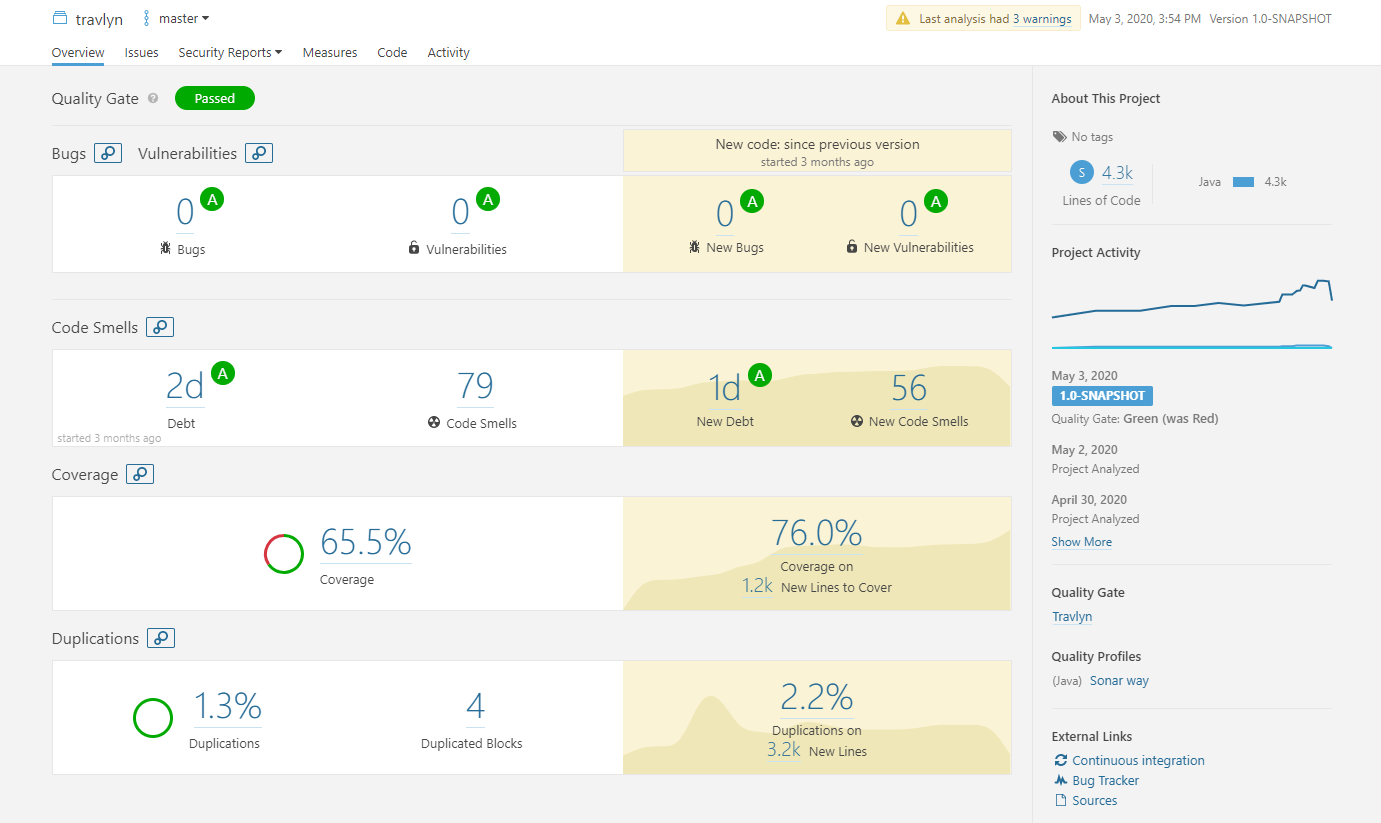
\includegraphics[width=1\textwidth]{images/sonar_passed_QG.png}
		\caption{Evaluation des Codes im Hinblick auf das Quality Gate in SonarQube}
		\label{fig:soarqube_QG}
	\end{figure}
	
	
	
	\subsection{Datenquellen}
	Aufgrund der begrenzten Ressourcen war die Auswahl der Datenquellen für dieses Projekt besonders kritisch: Es sollten keine Kosten anfallen und schwierige Lizenzfragen vermieden werden, um die Möglichkeit einer späteren Veröffentlichung der Applikation zu schaffen. Wie bereits in \autoref{sec:datengrundlage} beschrieben wurden die Quellen für \acs{POI}s und weiteren Informationen wie Kartendaten nach den gestellten Zielen ausgewählt. Nach Abschluss des Projekts ist festzuhalten, dass der Großteil der funktionalen Anforderungen mit diesen teilweise begrenzten Informationsquellen umgesetzt werden konnte (siehe \autoref{sec:funktional_evaluation}).
	
	\vspace{0.25cm}
	
	Neben der Auswahl der Datenquellen wurde auch die Auswahl der verwendeten Bibliotheken und Frameworks aufgrund dieser Ziele getroffen. So wurde sich z.B. explizit gegen ein UI Framework zur Visualisierung der Routenführung entschieden, welches nur für einen sehr begrenzten Nutzerkreis im Monat kostenlos gewesen wäre und es wurde eine eigene Implementation erstellt, welche die Crowd Sourced Daten von \acs{ORS} verwendet und visualisiert. Falls es geeignete Open Source Bibliotheken für das betreffende Thema gab, wurden diese eingesetzt, um den Aufwand einer eigenen Implementation zu sparen.
	
	\vspace{0.25cm}
	
	Aufgrund der Durchsetzung der oben genannten Maßnahmen könnte die App im aktuellen Zustand von rechtlicher Perspektive sicher veröffentlicht werden und auch für kommerzielle Zwecke genutzt werden, ohne das Risiko von Ansprüchen der Datenanbieter einzugehen. Trotz dieser Einschränkungen sind ansprechende Nutzungsmöglichkeiten entstanden, denen es nicht an Daten oder Funktionalität mangelt. Damit sind die Ziele für Datenquellen in diesem Projekt vollständig erfüllt.